\chapter{System Testing}
\label{chp:system_test}
\par There are three main components in this project system. There are \gls{rpi} residential access point, central management server and mobile application. So in this chapter test process will cover these three parts of the system.

\section{Testing on \gls{rpi}}
\par To test the system on \gls{rpi}, the working place shown in Figure \ref{fig:rpi_test} needs to be set up. Since the \gls{rpi} using in this project has only two bulit \gls{usb} port, one is taken by Wireless-G \gls{usb} Dongle. Then it is necessary to use an \gls{usb} hub to provide two more \gls{usb} port for keyboard and mouse to connect with. It is important that the \gls{usb} hub connected with \gls{rpi} is not require too high power voltage from \gls{rpi} because the power voltage is quite limited on \gls{rpi} board. Furthermore, the power cable of \gls{rpi} need to be check if it can be used for higher voltage power adapter because some time the normal data transition micro-usb cable is not enough to power up the \gls{rpi} device. To make the test and development of this project convenient, a \gls{hdmi} cable is used for \gls{rpi} to output display signal to the monitor. At last, the ethernet cable is required to give the \gls{rpi} access to the internet.

\begin{figure}
	\centering
    	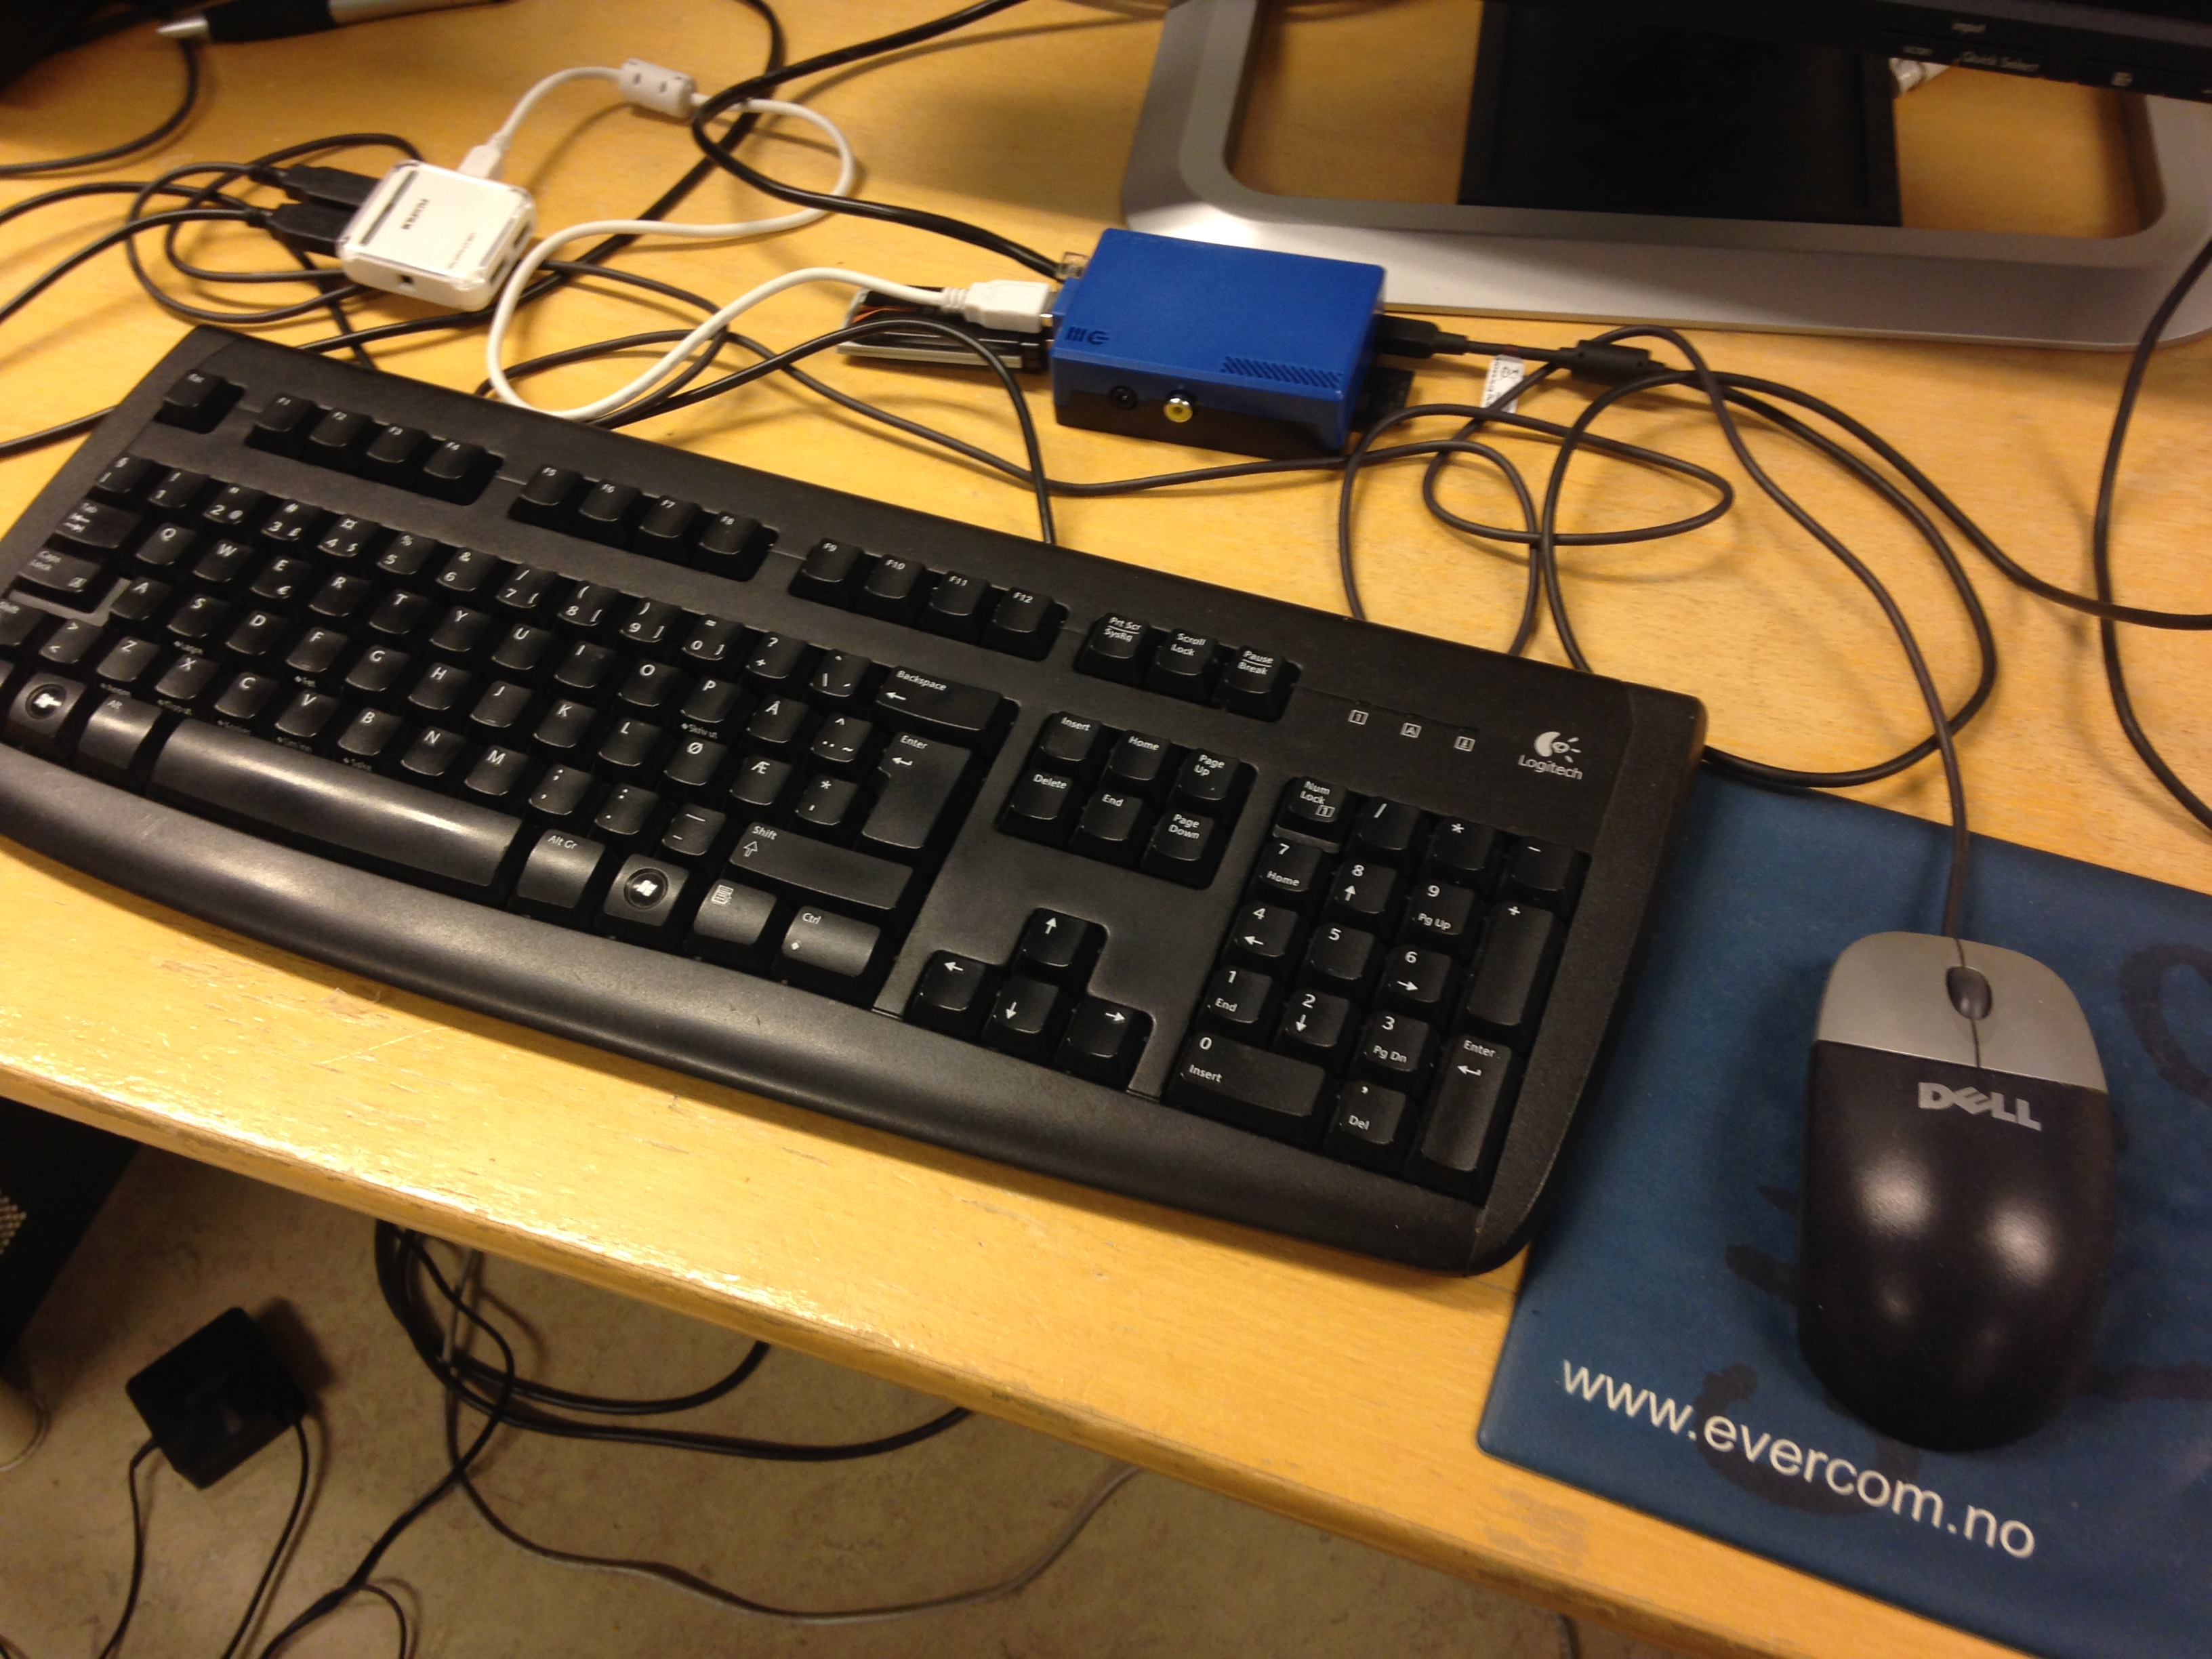
\includegraphics[width=0.80\textwidth,natwidth=610,natheight=642]{figs/rpi_test.JPG}
  	\caption{RPI Test Working Place}
  	\label{fig:rpi_test}
\end{figure}

\par The two python scripts partly shown in Code Snippet \ref{code:configserver_py} in Appendix \ref{chp:appendix} and on the Github repository \url{https://github.com/br1anchen/WifiAccess_RPIConfigurationServer/blob/master/transproxy.py} should be executed and keep running on \gls{rpi}. The full version of source code can be found on the Github repository \url{https://github.com/br1anchen/WifiAccess_RPIConfigurationServer}. The method of testing access point system on \gls{rpi} is to change the database of the client table (shown in the Figure \ref{fig:database_request}) on the central management server. The columns, 'json\_permission' and 'update\_flag' in the client table need to be changed to triggered the changing access right process for the corresponding client on the \gls{rpi}. For example, in the Figure \ref{fig:database_request}, the client 'BrianPC' is with the 'json\_permission' value '\{"permissions":\{"access":\{"allow":true\}\}\}' and the 'update\_flag' value '1'. It means that this client is approved by administrator and need to be updated its \gls{ip} address lease on the \gls{rpi} residential access point. For the test purpose, the 'json\_permission' value can be changed as '\{"permissions":\{"access":\{"allow":false\}\}\}' and keep the 'update\_flag' value still as '1'. Then the \gls{rpi} will know that this device is not allowed to access the residential network anymore, will make the blocking process for it.

\par The feedback of testing on \gls{rpi} shows that it is not easy for normal user to set up this internet access control system. And since the running process log only can be shown on external monitor by \gls{rpi}, the running scripts on the \gls{rpi} has no way to notify the normal user if there is error or failure of the running process. The suggested solution of this feedback will be discussed in Chapter \ref{chp:future_work}.

\begin{figure}
	\centering
    	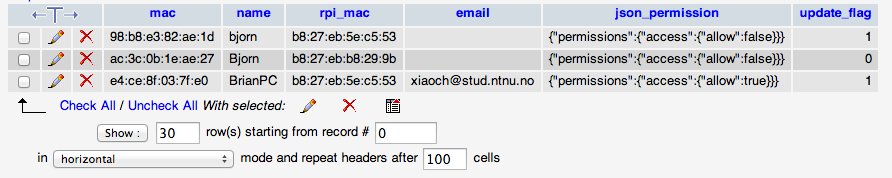
\includegraphics[width=0.80\textwidth,natwidth=610,natheight=642]{figs/database_request.png}
  	\caption{Client Database Table on Central Management Server}
  	\label{fig:database_request}
\end{figure}

\section{Testing on Central Management Server}
\par Because in this project, we make the improvement for login mechanism and E-mail notification for Central Management Server.So the test will be done for these two main feature of the Central Management Server.

\subsection{Login Mechanism Testing}
\par The login process communication between mobile application and central management server is \gls{http} post request with some user information on the request payload. The test for this feature will use a Chrome browser extension application called Advanced Rest Client to demonstrate the \gls{http} post request from the mobile application. The concept of Advanced Rest Client application is based on cURL\cite{curl} command, which is a computer software project providing a library and command-line tool for transferring data using various protocols. The working process to test login mechanism on central management server is shown in the Figure \ref{fig:restclient_test}. Because the user information data need to be encoded by Base64, then some online Base64 encoder web service is also used in this project for testing quite often, such as \url{http://www.base64encode.org/}. In Figure \ref{fig:restclient_test}, the use of Advanced Rest Client application is quite clear that it allows user to edit the value in the \gls{http} request header and payload. It helps the development and testing a lot.
\begin{figure}
	\centering
    	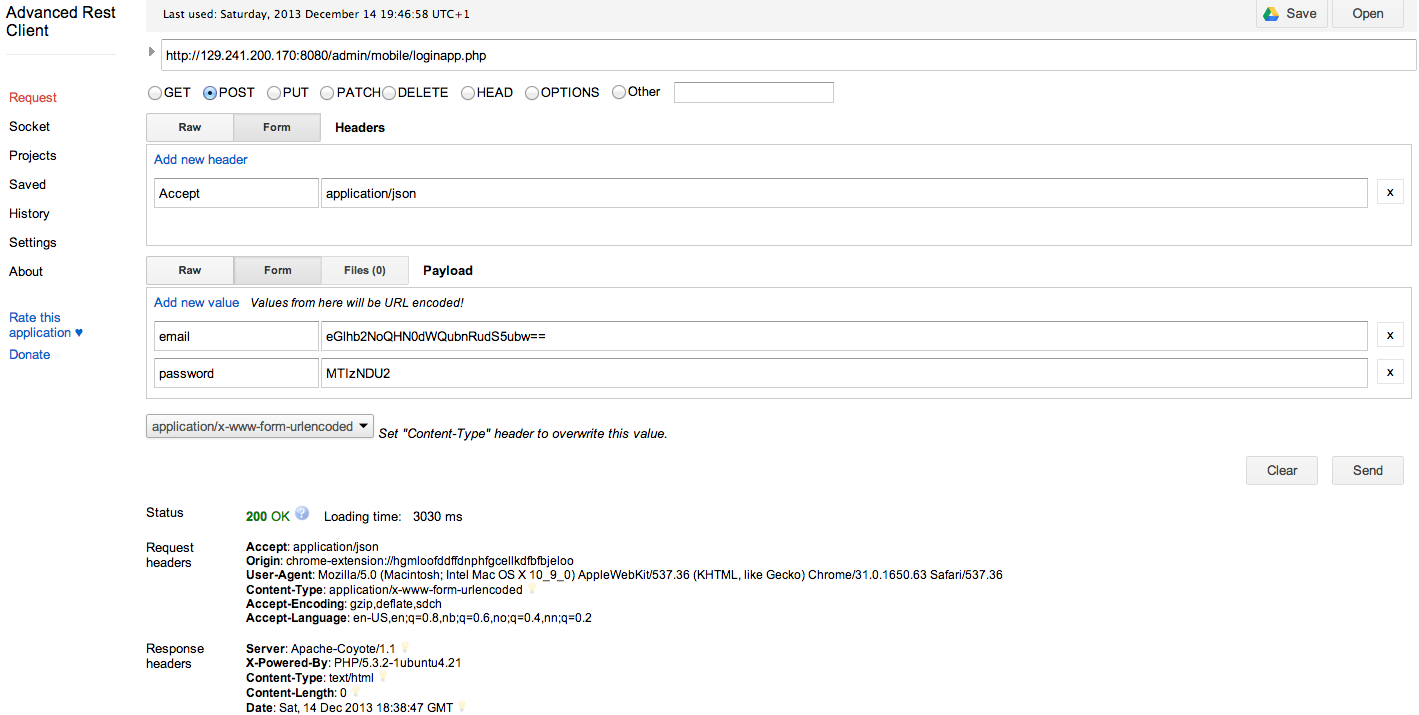
\includegraphics[width=0.80\textwidth,natwidth=610,natheight=642]{figs/restclient_test.png}
  	\caption{Advanced Rest Client Chrome Extension App for Central Management Server Test}
  	\label{fig:restclient_test}
\end{figure}

\par For testing the login mechanism on the central management server, the changing of the user information(for mobile manager client) database is also necessary. The Figure \ref{fig:database_user} is the administrator page of phpmyadmin for User database table on the central management server. By using phpmyadmin, the work to observe the changes of database and modify the database content or structure is much more easier than the previous master project.
\par The feedback of testing for login mechanism shows that it is a good solution to make the communication between mobile client and server more security than previous master project.And it makes the central management server hide behind the font side of the communication channel.
\begin{figure}
	\centering
    	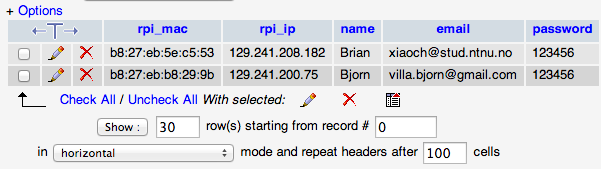
\includegraphics[width=0.80\textwidth,natwidth=610,natheight=642]{figs/database_user.png}
  	\caption{User Database Table on Central Management Server}
  	\label{fig:database_user}
\end{figure}

\subsection{E-mail notification}
\par To test the e-mail notification process of central management server is quite easy because the client request page shown in Figure \ref{fig:wifi_request_page} described in Chapter \ref{chp:system_description} can be used multiple times on one connected device in the network. It is reasonable since if the user is allowed in the residential network, then it should allow them to get the request result no matter it is approving or blocking. Then every time the client make the access request to the central management server, corresponding administrator need be notified by the E-mail from system. Although the weakness of the Brute-force attack will happen because of this process way, but by fixing the server work load case it should be handled quite well, this case will be more discussed in the Chapter \ref{chp:future_work} based on the feedback from the testing.
\par Through the testing of E-mail notification mechanism, the responsible administrator will get E-mail from the system E-mail address like the mail shown in Figure \ref{fig:request_note_mail}.
\begin{figure}
	\centering
    	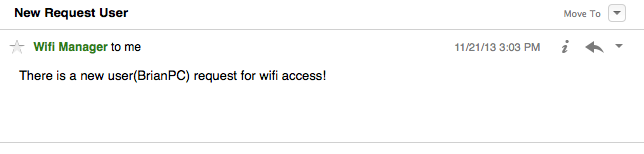
\includegraphics[width=0.80\textwidth,natwidth=610,natheight=642]{figs/request_note_mail.png}
  	\caption{Notification E-mail for Administrator}
  	\label{fig:request_note_mail}
\end{figure}
\par The feedback of this test shows that it is nice way to replace with the normal push notification function since there is no Apple developer account available in this prototype project.

\section{Testing on Mobile Application}
\par Because the simplicity of the mobile application, there is no test framework using during the development.The testing on mobile application is more focus on manually test for all the user behavior function on the mobile application. In this project, testing is on \gls{ios} mobile application. Since the time of development of this application is during the transition from old mobile operating system to new mobile operating system by Apple, more tests for application performance on different \gls{ios} platform.
\par Because of the limitation of different \gls{ios} devices with different versions of \gls{ios}, testing of mobile application has to be done on the simulator to get test result. Xcode \gls{ide} provides different simulators running different versions of \gls{ios} operating system. It also provides different versions of mobile \gls{cpu} like 32-bit and 64-bit on different simulators. The functionality testing is working on different simulators with different assert. According the result of testing, the \gls{ios} Wifi Manager mobile application is working well on all different kinds of simulators. The performance result of different simulators test shows that all the test have almost the same performance on all kinds of simulators. The reason for that, it is mainly because of the simplicity of the application and not physical devices running different versions of \gls{ios}.